\chapter{Marco te\'orico}
\label{Chapter2}

En este capítulo se presenta una visión general de la bibliografía relacionada al objetivo del presente trabajo. En la
primera sección se detalla una revisión de trabajos relacionados. En ... % TODO: completar

\section{Reconocimiento de d\'igitos}
\lipsum[1]

\section{Redes Neuronales}
\lipsum[1]

\subsection{Redes densas}
\lipsum[1]
% TODO: hablar de pre-train y fine-tuning

\subsection{Convolucionales}
\lipsum[1]

\subsection{Arquitecturas}
\lipsum[1]

\subsubsection{LeNet}
\lipsum[1]

\subsubsection{ResNet}
\lipsum[1]

\section{Adaptaci\'on de Dominio}
El {\it pre-entrenamiento} y el {\it fine-tuning} han mejorado considerablemente el estado del arte para diversos
problemas y aplicaciones del machine learning, incluso las redes profundas pre-entrenadas pueden adaptarse fácilmente a
tareas donde se cuenta con una pequeña cantidad de datos etiquetados. Sin embargo, en muchos escenarios prácticos, no
hay datos de entrenamiento etiquetados y, por lo tanto, existe la necesidad de transferir el aprendizaje de una red
profunda desde un dominio de origen en el que se dispone de datos de entrenamiento etiquetados a un dominio de destino
en el que solo existen datos sin etiquetar \parencite{glorot2011domain}. En esta situación, los modelos profundos siguen sufriendo degradaciones de rendimiento debido
al cambio de distribución \parencite{quinonero2008dataset}. Por lo tanto, se propone la {\it adaptación de dominio} para reducir el cambio de
distribución entre los dominios de entrenamiento y de prueba \parencite{jiang2022machine}.

Se han propuesto muchos métodos para la adaptación de dominios, ya sea ponderando o seleccionando muestras del dominio
de origen \parencite{sugiyama2007direct} o buscando una transformación de la distribución de origen a la distribución de destino \parencite{gong2013connecting}. Esta tesis analizar\'a algunos de los m\'etodos m\'as actuales del ultimo caso.

\subsection{Domain Adversarial Neural Network}
Un gran hito al momento de modelar distribuciones es la Red Generativa Adversaria {\it GAN} \parencite{goodfellow2020generative}. Inspirada en estas arquitecturas GAN, la Red Neural Adversaria de Dominio {\it DANN} \parencite{ganin2016domain} consta de dos redes en la adaptación del dominio (figura \ref{fig:dann-esquema}). La primera es
la discriminadora de dominios $\mathcal{D}$ entrenada para distinguir las características de origen de las de destino y
la segunda es una generadora de características $\mathcal{G}$ que se entrena para confundir a $\mathcal{D}$ y
simult\'aneamente ayudar a la red clasificadora $\mathcal{C}$.

\begin{figure}[H]
    \centering

    \tikzset{every picture/.style={line width=0.75pt}} %set default line width to 0.75pt        

    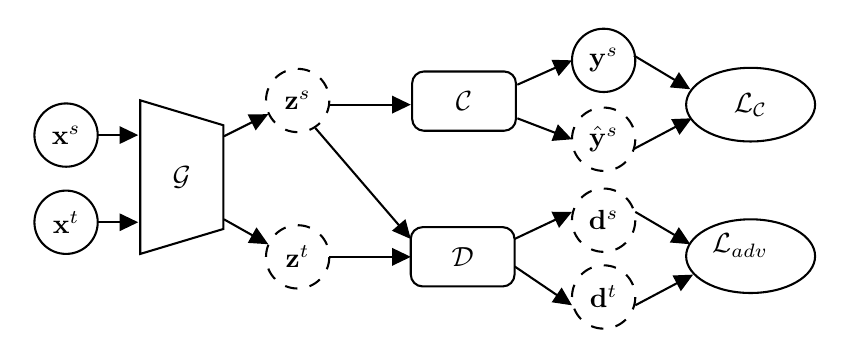
\begin{tikzpicture}[x=0.75pt,y=0.75pt,yscale=-1,xscale=1]
        \draw   (39,64.75) .. controls (39,56.33) and (45.83,49.5) .. (54.25,49.5) .. controls (62.67,49.5) and (69.5,56.33) .. (69.5,64.75) .. controls (69.5,73.17) and (62.67,80) .. (54.25,80) .. controls (45.83,80) and (39,73.17) .. (39,64.75) -- cycle ;

        \draw   (39,106.75) .. controls (39,98.33) and (45.83,91.5) .. (54.25,91.5) .. controls (62.67,91.5) and (69.5,98.33) .. (69.5,106.75) .. controls (69.5,115.17) and (62.67,122) .. (54.25,122) .. controls (45.83,122) and (39,115.17) .. (39,106.75) -- cycle ;

        \draw   (90,48) -- (130,60) -- (130,110) -- (90,122) -- cycle ;

        \draw    (69.5,64.75) -- (86,64.75) ;
        \draw [shift={(89,64.75)}, rotate = 180] [fill={rgb, 255:red, 0; green, 0; blue, 0 }  ][line width=0.08]  [draw opacity=0] (8.93,-4.29) -- (0,0) -- (8.93,4.29) -- cycle    ;
        \draw  [dash pattern={on 4.5pt off 4.5pt}] (150.58,48.08) .. controls (150.58,39.66) and (157.41,32.83) .. (165.83,32.83) .. controls (174.26,32.83) and (181.08,39.66) .. (181.08,48.08) .. controls (181.08,56.51) and (174.26,63.33) .. (165.83,63.33) .. controls (157.41,63.33) and (150.58,56.51) .. (150.58,48.08) -- cycle ;

        \draw  [dash pattern={on 4.5pt off 4.5pt}] (150.58,123.42) .. controls (150.58,114.99) and (157.41,108.17) .. (165.83,108.17) .. controls (174.26,108.17) and (181.08,114.99) .. (181.08,123.42) .. controls (181.08,131.84) and (174.26,138.67) .. (165.83,138.67) .. controls (157.41,138.67) and (150.58,131.84) .. (150.58,123.42) -- cycle ;

        \draw   (221,39.81) .. controls (221,36.65) and (223.56,34.1) .. (226.71,34.1) -- (265.29,34.1) .. controls (268.44,34.1) and (271,36.65) .. (271,39.81) -- (271,56.95) .. controls (271,60.11) and (268.44,62.67) .. (265.29,62.67) -- (226.71,62.67) .. controls (223.56,62.67) and (221,60.11) .. (221,56.95) -- cycle ;

        \draw   (220.33,114.81) .. controls (220.33,111.65) and (222.89,109.1) .. (226.05,109.1) -- (264.62,109.1) .. controls (267.77,109.1) and (270.33,111.65) .. (270.33,114.81) -- (270.33,131.95) .. controls (270.33,135.11) and (267.77,137.67) .. (264.62,137.67) -- (226.05,137.67) .. controls (222.89,137.67) and (220.33,135.11) .. (220.33,131.95) -- cycle ;

        \draw  [dash pattern={on 4.5pt off 4.5pt}] (298,105.75) .. controls (298,97.33) and (304.83,90.5) .. (313.25,90.5) .. controls (321.67,90.5) and (328.5,97.33) .. (328.5,105.75) .. controls (328.5,114.17) and (321.67,121) .. (313.25,121) .. controls (304.83,121) and (298,114.17) .. (298,105.75) -- cycle ;

        \draw  [dash pattern={on 4.5pt off 4.5pt}] (298,142.75) .. controls (298,134.33) and (304.83,127.5) .. (313.25,127.5) .. controls (321.67,127.5) and (328.5,134.33) .. (328.5,142.75) .. controls (328.5,151.17) and (321.67,158) .. (313.25,158) .. controls (304.83,158) and (298,151.17) .. (298,142.75) -- cycle ;

        \draw   (353,123.08) .. controls (353,113.28) and (366.91,105.33) .. (384.06,105.33) .. controls (401.22,105.33) and (415.13,113.28) .. (415.13,123.08) .. controls (415.13,132.89) and (401.22,140.83) .. (384.06,140.83) .. controls (366.91,140.83) and (353,132.89) .. (353,123.08) -- cycle ;

        \draw   (298,28.75) .. controls (298,20.33) and (304.83,13.5) .. (313.25,13.5) .. controls (321.67,13.5) and (328.5,20.33) .. (328.5,28.75) .. controls (328.5,37.17) and (321.67,44) .. (313.25,44) .. controls (304.83,44) and (298,37.17) .. (298,28.75) -- cycle ;
        \draw  [dash pattern={on 4.5pt off 4.5pt}] (298,66.75) .. controls (298,58.33) and (304.83,51.5) .. (313.25,51.5) .. controls (321.67,51.5) and (328.5,58.33) .. (328.5,66.75) .. controls (328.5,75.17) and (321.67,82) .. (313.25,82) .. controls (304.83,82) and (298,75.17) .. (298,66.75) -- cycle ;
        \draw   (353,50.08) .. controls (353,40.28) and (366.91,32.33) .. (384.06,32.33) .. controls (401.22,32.33) and (415.13,40.28) .. (415.13,50.08) .. controls (415.13,59.89) and (401.22,67.83) .. (384.06,67.83) .. controls (366.91,67.83) and (353,59.89) .. (353,50.08) -- cycle ;
        \draw    (69.5,106.75) -- (86,106.75) ;
        \draw [shift={(89,106.75)}, rotate = 180] [fill={rgb, 255:red, 0; green, 0; blue, 0 }  ][line width=0.08]  [draw opacity=0] (8.93,-4.29) -- (0,0) -- (8.93,4.29) -- cycle    ;
        \draw    (130.33,65.33) -- (148.98,56.01) ;
        \draw [shift={(151.67,54.67)}, rotate = 153.43] [fill={rgb, 255:red, 0; green, 0; blue, 0 }  ][line width=0.08]  [draw opacity=0] (8.93,-4.29) -- (0,0) -- (8.93,4.29) -- cycle    ;
        \draw    (130.33,105.33) -- (149.05,115.86) ;
        \draw [shift={(151.67,117.33)}, rotate = 209.36] [fill={rgb, 255:red, 0; green, 0; blue, 0 }  ][line width=0.08]  [draw opacity=0] (8.93,-4.29) -- (0,0) -- (8.93,4.29) -- cycle    ;
        \draw    (181.08,50.08) -- (217.33,50.08) ;
        \draw [shift={(220.33,50.08)}, rotate = 180] [fill={rgb, 255:red, 0; green, 0; blue, 0 }  ][line width=0.08]  [draw opacity=0] (8.93,-4.29) -- (0,0) -- (8.93,4.29) -- cycle    ;
        \draw    (181.08,123.42) -- (217.33,123.42) ;
        \draw [shift={(220.33,123.42)}, rotate = 180] [fill={rgb, 255:red, 0; green, 0; blue, 0 }  ][line width=0.08]  [draw opacity=0] (8.93,-4.29) -- (0,0) -- (8.93,4.29) -- cycle    ;
        \draw    (174.33,61.33) -- (218.38,112.54) ;
        \draw [shift={(220.33,114.81)}, rotate = 229.3] [fill={rgb, 255:red, 0; green, 0; blue, 0 }  ][line width=0.08]  [draw opacity=0] (8.93,-4.29) -- (0,0) -- (8.93,4.29) -- cycle    ;
        \draw    (270.33,114.81) -- (295.29,103.03) ;
        \draw [shift={(298,101.75)}, rotate = 154.73] [fill={rgb, 255:red, 0; green, 0; blue, 0 }  ][line width=0.08]  [draw opacity=0] (8.93,-4.29) -- (0,0) -- (8.93,4.29) -- cycle    ;
        \draw    (270.33,128) -- (295.52,145.07) ;
        \draw [shift={(298,146.75)}, rotate = 214.13] [fill={rgb, 255:red, 0; green, 0; blue, 0 }  ][line width=0.08]  [draw opacity=0] (8.93,-4.29) -- (0,0) -- (8.93,4.29) -- cycle    ;
        \draw    (328.5,101.75) -- (352.41,115.81) ;
        \draw [shift={(355,117.33)}, rotate = 210.46] [fill={rgb, 255:red, 0; green, 0; blue, 0 }  ][line width=0.08]  [draw opacity=0] (8.93,-4.29) -- (0,0) -- (8.93,4.29) -- cycle    ;
        \draw    (328.5,146.75) -- (353.68,133.4) ;
        \draw [shift={(356.33,132)}, rotate = 152.08] [fill={rgb, 255:red, 0; green, 0; blue, 0 }  ][line width=0.08]  [draw opacity=0] (8.93,-4.29) -- (0,0) -- (8.93,4.29) -- cycle    ;
        \draw    (271.67,40.48) -- (295.26,29.97) ;
        \draw [shift={(298,28.75)}, rotate = 156] [fill={rgb, 255:red, 0; green, 0; blue, 0 }  ][line width=0.08]  [draw opacity=0] (8.93,-4.29) -- (0,0) -- (8.93,4.29) -- cycle    ;
        \draw    (271.67,56.67) -- (295.2,65.68) ;
        \draw [shift={(298,66.75)}, rotate = 200.95] [fill={rgb, 255:red, 0; green, 0; blue, 0 }  ][line width=0.08]  [draw opacity=0] (8.93,-4.29) -- (0,0) -- (8.93,4.29) -- cycle    ;
        \draw    (327.83,26.42) -- (352.43,41.13) ;
        \draw [shift={(355,42.67)}, rotate = 210.89] [fill={rgb, 255:red, 0; green, 0; blue, 0 }  ][line width=0.08]  [draw opacity=0] (8.93,-4.29) -- (0,0) -- (8.93,4.29) -- cycle    ;
        \draw    (327.83,71.42) -- (353.02,58.07) ;
        \draw [shift={(355.67,56.67)}, rotate = 152.08] [fill={rgb, 255:red, 0; green, 0; blue, 0 }  ][line width=0.08]  [draw opacity=0] (8.93,-4.29) -- (0,0) -- (8.93,4.29) -- cycle    ;

        \draw (165.83,123.42) node   [align=left] {\begin{minipage}[lt]{21.08pt}\setlength\topsep{0pt}
                \begin{center}
                    $\mathbf{z}^t$
                \end{center}

            \end{minipage}};
        \draw (165.83,48.08) node   [align=left] {\begin{minipage}[lt]{21.08pt}\setlength\topsep{0pt}
                \begin{center}
                    $\mathbf{z}^s$
                \end{center}

            \end{minipage}};
        \draw (245.33,123.56) node   [align=left] {\begin{minipage}[lt]{26.23pt}\setlength\topsep{0pt}
                \begin{center}
                    $\mathcal{D}$
                \end{center}

            \end{minipage}};
        \draw (246,48.56) node   [align=left] {\begin{minipage}[lt]{26.23pt}\setlength\topsep{0pt}
                \begin{center}
                    $\mathcal{C}$
                \end{center}

            \end{minipage}};
        \draw (110,85) node   [align=left] {\begin{minipage}[lt]{22.78pt}\setlength\topsep{0pt}
                \begin{center}
                    $\mathcal{G}$
                \end{center}

            \end{minipage}};
        \draw (54.25,106.75) node   [align=left] {\begin{minipage}[lt]{21.08pt}\setlength\topsep{0pt}
                \begin{center}
                    $\mathbf{x}^t$
                \end{center}

            \end{minipage}};
        \draw (54.25,64.75) node   [align=left] {\begin{minipage}[lt]{21.08pt}\setlength\topsep{0pt}
                \begin{center}
                    $\mathbf{x}^s$
                \end{center}

            \end{minipage}};
        \draw (313.25,142.75) node   [align=left] {\begin{minipage}[lt]{21.08pt}\setlength\topsep{0pt}
                \begin{center}
                    $\mathbf{d}^t$
                \end{center}

            \end{minipage}};
        \draw (313.25,105.75) node   [align=left] {\begin{minipage}[lt]{21.08pt}\setlength\topsep{0pt}
                \begin{center}
                    $\mathbf{d}^s$
                \end{center}

            \end{minipage}};
        \draw (379,118) node   [align=left] {\begin{minipage}[lt]{32.64pt}\setlength\topsep{0pt}
                \begin{center}
                    $\mathcal{L}_{adv}$
                \end{center}

            \end{minipage}};
        \draw (313.25,28.75) node   [align=left] {\begin{minipage}[lt]{21.08pt}\setlength\topsep{0pt}
                \begin{center}
                    $\mathbf{y}^s$
                \end{center}

            \end{minipage}};
        \draw (313.25,66.75) node   [align=left] {\begin{minipage}[lt]{21.08pt}\setlength\topsep{0pt}
                \begin{center}
                    $\hat{\mathbf{y}}^s$
                \end{center}

            \end{minipage}};
        \draw (384.06,50.08) node   [align=left] {\begin{minipage}[lt]{32.64pt}\setlength\topsep{0pt}
                \begin{center}
                    $\mathcal{L}_{\mathcal{C}}$
                \end{center}
            \end{minipage}};
    \end{tikzpicture}

    \caption{Esquema de las {\it DANN}. Los supra indices $s$ y $t$ indican si los datos son del origen o destino respectivamente.
        Los c\'irculos con l\'ineas rayadas son salidas de los modelos mientras que los c\'irculos de l\'ineas s\'olidas son datos conocidos.}
    \label{fig:dann-esquema}
\end{figure}

El objetivo de {\it DANN} consiste en minimizar funci\'on de p\'erdida que depende de $\mathcal{L}_\mathcal{C}$ y
$\mathcal{L}_{adv}$. $\mathcal{L}_\mathcal{C}$ mide el error que posee la red en la clasificaci\'on de los datos de
origen y viene dada por el {\it cross-entropy} $\mathcal{L}_{CE}$ aplicado a la salida de la red $\mathcal{C}$. El
objetivo de $\mathcal{D}$ ser\'a la descripta en la ecuaci\'on \ref{eq:dann-loss-clasificadora}:

\begin{align}
    \min_{\mathcal{C}} \mathcal{L}_\mathcal{C}(\mathbf{x}^s, \mathbf{y}^s) & = \mathcal{L}_{CE}(C(\mathcal{G}(\mathbf{x}^s)), \mathbf{y}^s) \nonumber \\
                                                                           & = \mathcal{L}_{CE}(C(\mathbf{z}^s), \mathbf{y}^s) \nonumber              \\
                                                                           & = \mathcal{L}_{CE}(\hat{\mathbf{y}}^s, \mathbf{y}^s)
    \label{eq:dann-loss-clasificadora}
\end{align}

La funci\'on de p\'erdida de $\mathcal{D}$ viene dada por la ecuaci\'on \ref{eq:dann-loss-discriminadora}, donde
$\mathbb{E}_{\mathbf{x}^s \sim \mathcal{\hat{S}}}$ y $\mathbb{E}_{\mathbf{x}^t \sim \mathcal{\hat{T}}}$ representan la
proporci\'on esperada de datos de origen $\mathcal{\hat{S}}$ y destino $\mathcal{\hat{T}}$ respectivamente.

\begin{align}
    \max_{\mathcal{D}} \mathcal{L}_{adv}(\mathbf{x}^s, \mathbf{x}^t) & = \mathbb{E}_{\mathbf{x}^s \sim \mathcal{\hat{S}}}\log[\mathcal{D}(\mathcal{G}(\mathbf{x}^s))] + \mathbb{E}_{\mathbf{x}^t \sim \mathcal{\hat{T}}}\log[1-\mathcal{D}(\mathcal{G}(\mathbf{x}^t))] \nonumber \\
                                                                     & = \mathbb{E}_{\mathbf{x}^s \sim \mathcal{\hat{S}}}\log[\mathcal{D}(\mathbf{z}^s)] + \mathbb{E}_{\mathbf{x}^t \sim \mathcal{\hat{T}}}\log[1-\mathcal{D}(\mathbf{z}^t)] \nonumber                           \\
                                                                     & = \mathbb{E}_{\mathbf{x}^s \sim \mathcal{\hat{S}}}\log[\mathbf{d}^s] + \mathbb{E}_{\mathbf{x}^t \sim \mathcal{\hat{T}}}\log[1-\mathbf{d}^t]
    \label{eq:dann-loss-discriminadora}
\end{align}

Por lo tanto, el objetivo de un modelo {\it DANN} viene dado por la ecuaci\'on \ref{eq:dann-objetivo}. Donde $\lambda$
es un hiper-par\'ametro a optimizar que regula el trade-off entre la clasificaci\'on y la discriminaci\'on adversaria.
La minimización de $\mathcal{L}_\mathcal{C}$ dará lugar a representaciones discriminables, mientras que la disminución
de $\mathcal{L}_\mathcal{D}$ dará lugar a representaciones transferibles.

\begin{align}
    \min_{\mathcal{G},\mathcal{C}} \mathcal{L}_\mathcal{C}(\mathbf{x}^s, \mathbf{y}^s) + \lambda \mathcal{L}_{adv}(\mathbf{x}^s, \mathbf{x}^t)
    \label{eq:dann-objetivo}
\end{align}

\subsection{Adversarial Discriminative Domain Adaptation}
Las redes Adversarial Discriminative Domain Adaptation {\it ADDA} \parencite{tzeng2017adversarial} surgen a partir de las {\it DANN} debido a que su estrategia de optimización podría no
funcionar bien en la práctica debido a la desvanecimiento del gradiente, que también es un problema importante en el
entrenamiento de GANs. Por ejemplo, cuando el espacio latente de destino generado $\mathbf{z}^t$ es extremadamente
distinguible del de origen tal que $\mathcal{D}(\mathbf{z}^t)=0$, el gradiente es peque\~{n}o y vice versa. Esto
provoca que la optimizaci\'on de $\mathcal{G}$ sea extremadamente dif\'icil.

Las redes {\it ADDA} separan la optimizaci\'on de $\mathcal{G}$ y de $\mathcal{D}$ en dos objetivos separados (figura
\ref{fig:adda-esquema}) siendo el primero el pre-entrenamiento de $\mathcal{G}_s$ y $\mathcal{C}$ en los datos de
origen y el otro siendo la adaptaci\'on adversaria de una $\mathcal{G}_t$ utilizando a $\mathcal{G}_s$ pre-entrenada y
$\mathcal{D}$.

\begin{figure}[H]
    \centering

    \tikzset{every picture/.style={line width=0.75pt}} %set default line width to 0.75pt        

    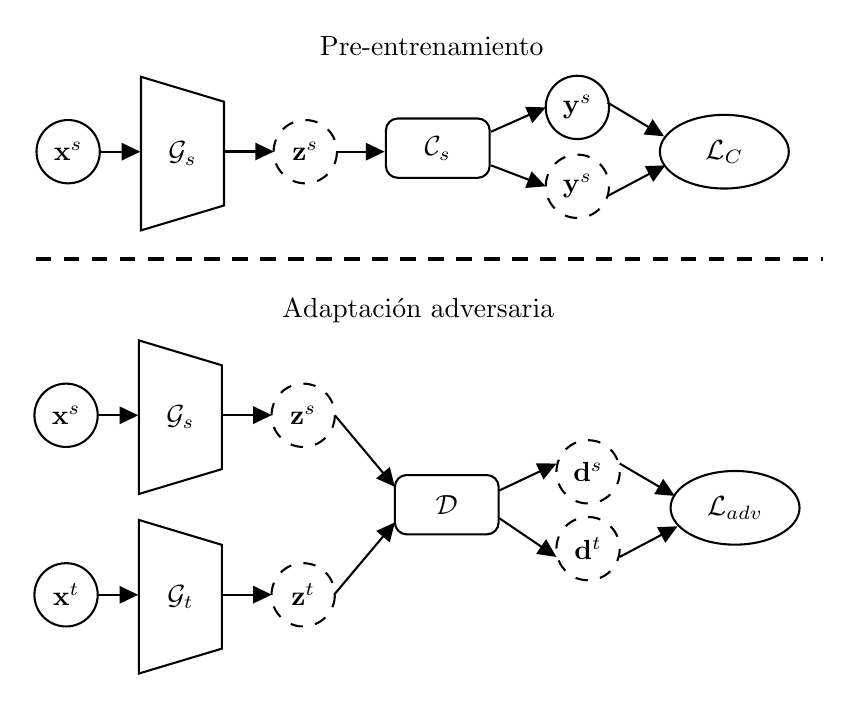
\begin{tikzpicture}[x=0.75pt,y=0.75pt,yscale=-1,xscale=1]
        %uncomment if require: \path (0,385); %set diagram left start at 0, and has height of 385

        \draw   (20.33,88.25) .. controls (20.33,79.83) and (27.16,73) .. (35.58,73) .. controls (44.01,73) and (50.83,79.83) .. (50.83,88.25) .. controls (50.83,96.67) and (44.01,103.5) .. (35.58,103.5) .. controls (27.16,103.5) and (20.33,96.67) .. (20.33,88.25) -- cycle ;

        \draw   (70.67,52.17) -- (110.67,64.17) -- (110.67,114.17) -- (70.67,126.17) -- cycle ;
        \draw    (50.83,88.25) -- (67.33,88.25) ;
        \draw [shift={(70.33,88.25)}, rotate = 180] [fill={rgb, 255:red, 0; green, 0; blue, 0 }  ][line width=0.08]  [draw opacity=0] (8.93,-4.29) -- (0,0) -- (8.93,4.29) -- cycle    ;
        \draw  [dash pattern={on 4.5pt off 4.5pt}] (134.58,88.25) .. controls (134.58,79.83) and (141.41,73) .. (149.83,73) .. controls (158.26,73) and (165.08,79.83) .. (165.08,88.25) .. controls (165.08,96.67) and (158.26,103.5) .. (149.83,103.5) .. controls (141.41,103.5) and (134.58,96.67) .. (134.58,88.25) -- cycle ;

        \draw   (188.67,77.98) .. controls (188.67,74.82) and (191.23,72.26) .. (194.38,72.26) -- (232.95,72.26) .. controls (236.11,72.26) and (238.67,74.82) .. (238.67,77.98) -- (238.67,95.12) .. controls (238.67,98.27) and (236.11,100.83) .. (232.95,100.83) -- (194.38,100.83) .. controls (191.23,100.83) and (188.67,98.27) .. (188.67,95.12) -- cycle ;
        \draw   (265.67,66.92) .. controls (265.67,58.49) and (272.49,51.67) .. (280.92,51.67) .. controls (289.34,51.67) and (296.17,58.49) .. (296.17,66.92) .. controls (296.17,75.34) and (289.34,82.17) .. (280.92,82.17) .. controls (272.49,82.17) and (265.67,75.34) .. (265.67,66.92) -- cycle ;
        \draw  [dash pattern={on 4.5pt off 4.5pt}] (265.67,104.92) .. controls (265.67,96.49) and (272.49,89.67) .. (280.92,89.67) .. controls (289.34,89.67) and (296.17,96.49) .. (296.17,104.92) .. controls (296.17,113.34) and (289.34,120.17) .. (280.92,120.17) .. controls (272.49,120.17) and (265.67,113.34) .. (265.67,104.92) -- cycle ;
        \draw   (320.67,88.25) .. controls (320.67,78.45) and (334.57,70.5) .. (351.73,70.5) .. controls (368.88,70.5) and (382.79,78.45) .. (382.79,88.25) .. controls (382.79,98.05) and (368.88,106) .. (351.73,106) .. controls (334.57,106) and (320.67,98.05) .. (320.67,88.25) -- cycle ;
        \draw    (111.33,88.17) -- (131.67,88.17) ;
        \draw [shift={(134.67,88.17)}, rotate = 180] [fill={rgb, 255:red, 0; green, 0; blue, 0 }  ][line width=0.08]  [draw opacity=0] (8.93,-4.29) -- (0,0) -- (8.93,4.29) -- cycle    ;
        \draw    (164.67,88.25) -- (185,88.25) ;
        \draw [shift={(188,88.25)}, rotate = 180] [fill={rgb, 255:red, 0; green, 0; blue, 0 }  ][line width=0.08]  [draw opacity=0] (8.93,-4.29) -- (0,0) -- (8.93,4.29) -- cycle    ;
        \draw    (239.33,78.64) -- (262.93,68.14) ;
        \draw [shift={(265.67,66.92)}, rotate = 156] [fill={rgb, 255:red, 0; green, 0; blue, 0 }  ][line width=0.08]  [draw opacity=0] (8.93,-4.29) -- (0,0) -- (8.93,4.29) -- cycle    ;
        \draw    (239.33,94.83) -- (262.87,103.84) ;
        \draw [shift={(265.67,104.92)}, rotate = 200.95] [fill={rgb, 255:red, 0; green, 0; blue, 0 }  ][line width=0.08]  [draw opacity=0] (8.93,-4.29) -- (0,0) -- (8.93,4.29) -- cycle    ;
        \draw    (295.5,64.58) -- (320.09,79.29) ;
        \draw [shift={(322.67,80.83)}, rotate = 210.89] [fill={rgb, 255:red, 0; green, 0; blue, 0 }  ][line width=0.08]  [draw opacity=0] (8.93,-4.29) -- (0,0) -- (8.93,4.29) -- cycle    ;
        \draw    (295.5,109.58) -- (320.68,96.24) ;
        \draw [shift={(323.33,94.83)}, rotate = 152.08] [fill={rgb, 255:red, 0; green, 0; blue, 0 }  ][line width=0.08]  [draw opacity=0] (8.93,-4.29) -- (0,0) -- (8.93,4.29) -- cycle    ;
        \draw   (19.33,215.25) .. controls (19.33,206.83) and (26.16,200) .. (34.58,200) .. controls (43.01,200) and (49.83,206.83) .. (49.83,215.25) .. controls (49.83,223.67) and (43.01,230.5) .. (34.58,230.5) .. controls (26.16,230.5) and (19.33,223.67) .. (19.33,215.25) -- cycle ;

        \draw   (69.67,179.17) -- (109.67,191.17) -- (109.67,241.17) -- (69.67,253.17) -- cycle ;
        \draw    (49.83,215.25) -- (66.33,215.25) ;
        \draw [shift={(69.33,215.25)}, rotate = 180] [fill={rgb, 255:red, 0; green, 0; blue, 0 }  ][line width=0.08]  [draw opacity=0] (8.93,-4.29) -- (0,0) -- (8.93,4.29) -- cycle    ;
        \draw  [dash pattern={on 4.5pt off 4.5pt}] (133.58,215.25) .. controls (133.58,206.83) and (140.41,200) .. (148.83,200) .. controls (157.26,200) and (164.08,206.83) .. (164.08,215.25) .. controls (164.08,223.67) and (157.26,230.5) .. (148.83,230.5) .. controls (140.41,230.5) and (133.58,223.67) .. (133.58,215.25) -- cycle ;

        \draw    (110.33,215.17) -- (130.67,215.17) ;
        \draw [shift={(133.67,215.17)}, rotate = 180] [fill={rgb, 255:red, 0; green, 0; blue, 0 }  ][line width=0.08]  [draw opacity=0] (8.93,-4.29) -- (0,0) -- (8.93,4.29) -- cycle    ;
        \draw    (164.08,215.25) -- (191.07,247.45) ;
        \draw [shift={(193,249.75)}, rotate = 230.03] [fill={rgb, 255:red, 0; green, 0; blue, 0 }  ][line width=0.08]  [draw opacity=0] (8.93,-4.29) -- (0,0) -- (8.93,4.29) -- cycle    ;
        \draw   (19.33,301.75) .. controls (19.33,293.33) and (26.16,286.5) .. (34.58,286.5) .. controls (43.01,286.5) and (49.83,293.33) .. (49.83,301.75) .. controls (49.83,310.17) and (43.01,317) .. (34.58,317) .. controls (26.16,317) and (19.33,310.17) .. (19.33,301.75) -- cycle ;

        \draw   (69.67,265.67) -- (109.67,277.67) -- (109.67,327.67) -- (69.67,339.67) -- cycle ;
        \draw    (49.83,301.75) -- (66.33,301.75) ;
        \draw [shift={(69.33,301.75)}, rotate = 180] [fill={rgb, 255:red, 0; green, 0; blue, 0 }  ][line width=0.08]  [draw opacity=0] (8.93,-4.29) -- (0,0) -- (8.93,4.29) -- cycle    ;
        \draw  [dash pattern={on 4.5pt off 4.5pt}] (133.58,301.75) .. controls (133.58,293.33) and (140.41,286.5) .. (148.83,286.5) .. controls (157.26,286.5) and (164.08,293.33) .. (164.08,301.75) .. controls (164.08,310.17) and (157.26,317) .. (148.83,317) .. controls (140.41,317) and (133.58,310.17) .. (133.58,301.75) -- cycle ;
        \draw    (110.33,301.67) -- (130.67,301.67) ;
        \draw [shift={(133.67,301.67)}, rotate = 180] [fill={rgb, 255:red, 0; green, 0; blue, 0 }  ][line width=0.08]  [draw opacity=0] (8.93,-4.29) -- (0,0) -- (8.93,4.29) -- cycle    ;
        \draw    (163.67,301.75) -- (191.07,269.19) ;
        \draw [shift={(193,266.89)}, rotate = 130.08] [fill={rgb, 255:red, 0; green, 0; blue, 0 }  ][line width=0.08]  [draw opacity=0] (8.93,-4.29) -- (0,0) -- (8.93,4.29) -- cycle    ;
        \draw   (193,249.75) .. controls (193,246.59) and (195.56,244.04) .. (198.71,244.04) -- (237.29,244.04) .. controls (240.44,244.04) and (243,246.59) .. (243,249.75) -- (243,266.89) .. controls (243,270.05) and (240.44,272.61) .. (237.29,272.61) -- (198.71,272.61) .. controls (195.56,272.61) and (193,270.05) .. (193,266.89) -- cycle ;

        \draw  [dash pattern={on 4.5pt off 4.5pt}] (270.83,242.5) .. controls (270.83,234.08) and (277.66,227.25) .. (286.08,227.25) .. controls (294.51,227.25) and (301.33,234.08) .. (301.33,242.5) .. controls (301.33,250.92) and (294.51,257.75) .. (286.08,257.75) .. controls (277.66,257.75) and (270.83,250.92) .. (270.83,242.5) -- cycle ;

        \draw  [dash pattern={on 4.5pt off 4.5pt}] (270.83,279.5) .. controls (270.83,271.08) and (277.66,264.25) .. (286.08,264.25) .. controls (294.51,264.25) and (301.33,271.08) .. (301.33,279.5) .. controls (301.33,287.92) and (294.51,294.75) .. (286.08,294.75) .. controls (277.66,294.75) and (270.83,287.92) .. (270.83,279.5) -- cycle ;

        \draw   (325.83,259.83) .. controls (325.83,250.03) and (339.74,242.08) .. (356.9,242.08) .. controls (374.05,242.08) and (387.96,250.03) .. (387.96,259.83) .. controls (387.96,269.64) and (374.05,277.58) .. (356.9,277.58) .. controls (339.74,277.58) and (325.83,269.64) .. (325.83,259.83) -- cycle ;

        \draw    (243.17,251.56) -- (268.12,239.78) ;
        \draw [shift={(270.83,238.5)}, rotate = 154.73] [fill={rgb, 255:red, 0; green, 0; blue, 0 }  ][line width=0.08]  [draw opacity=0] (8.93,-4.29) -- (0,0) -- (8.93,4.29) -- cycle    ;
        \draw    (243.17,264.75) -- (268.35,281.82) ;
        \draw [shift={(270.83,283.5)}, rotate = 214.13] [fill={rgb, 255:red, 0; green, 0; blue, 0 }  ][line width=0.08]  [draw opacity=0] (8.93,-4.29) -- (0,0) -- (8.93,4.29) -- cycle    ;
        \draw    (301.33,238.5) -- (325.25,252.56) ;
        \draw [shift={(327.83,254.08)}, rotate = 210.46] [fill={rgb, 255:red, 0; green, 0; blue, 0 }  ][line width=0.08]  [draw opacity=0] (8.93,-4.29) -- (0,0) -- (8.93,4.29) -- cycle    ;
        \draw    (301.33,283.5) -- (326.52,270.15) ;
        \draw [shift={(329.17,268.75)}, rotate = 152.08] [fill={rgb, 255:red, 0; green, 0; blue, 0 }  ][line width=0.08]  [draw opacity=0] (8.93,-4.29) -- (0,0) -- (8.93,4.29) -- cycle    ;
        \draw [line width=1.5]  [dash pattern={on 5.63pt off 4.5pt}]  (20,140) -- (399.5,140) ;

        \draw (280.92,66.92) node   [align=left] {\begin{minipage}[lt]{21.08pt}\setlength\topsep{0pt}
                \begin{center}
                    $\mathbf{y}^s$
                \end{center}
            \end{minipage}};
        \draw (280.92,104.92) node   [align=left] {\begin{minipage}[lt]{21.08pt}\setlength\topsep{0pt}
                \begin{center}
                    $\mathbf{y}^s$
                \end{center}
            \end{minipage}};
        \draw (351.73,88.25) node   [align=left] {\begin{minipage}[lt]{32.64pt}\setlength\topsep{0pt}
                \begin{center}
                    $\mathcal{L}_C$
                \end{center}
            \end{minipage}};
        \draw (149.83,88.25) node   [align=left] {\begin{minipage}[lt]{21.08pt}\setlength\topsep{0pt}
                \begin{center}
                    $\mathbf{z}^s$
                \end{center}
            \end{minipage}};
        \draw (35.58,88.25) node   [align=left] {\begin{minipage}[lt]{21.08pt}\setlength\topsep{0pt}
                \begin{center}
                    $\mathbf{x}^s$
                \end{center}
            \end{minipage}};
        \draw (90.67,89.17) node   [align=left] {\begin{minipage}[lt]{22.78pt}\setlength\topsep{0pt}
                \begin{center}
                    $\mathcal{G}_s$
                \end{center}
            \end{minipage}};
        \draw (213.67,86.73) node   [align=left] {\begin{minipage}[lt]{26.23pt}\setlength\topsep{0pt}
                \begin{center}
                    $\mathcal{C}_s$
                \end{center}
            \end{minipage}};
        \draw (89.67,216.17) node   [align=left] {\begin{minipage}[lt]{22.78pt}\setlength\topsep{0pt}
                \begin{center}
                    $\mathcal{G}_s$
                \end{center}
            \end{minipage}};
        \draw (148.83,215.25) node   [align=left] {\begin{minipage}[lt]{21.08pt}\setlength\topsep{0pt}
                \begin{center}
                    $\mathbf{z}^s$
                \end{center}
            \end{minipage}};
        \draw (34.58,215.25) node   [align=left] {\begin{minipage}[lt]{21.08pt}\setlength\topsep{0pt}
                \begin{center}
                    $\mathbf{x}^s$
                \end{center}
            \end{minipage}};
        \draw (89.67,302.67) node   [align=left] {\begin{minipage}[lt]{22.78pt}\setlength\topsep{0pt}
                \begin{center}
                    $\mathcal{G}_t$
                \end{center}
            \end{minipage}};
        \draw (34.58,301.75) node   [align=left] {\begin{minipage}[lt]{21.08pt}\setlength\topsep{0pt}
                \begin{center}
                    $\mathbf{x}^t$
                \end{center}
            \end{minipage}};
        \draw (148.83,301.75) node   [align=left] {\begin{minipage}[lt]{21.08pt}\setlength\topsep{0pt}
                \begin{center}
                    $\mathbf{z}^t$
                \end{center}
            \end{minipage}};
        \draw (218,258.5) node   [align=left] {\begin{minipage}[lt]{26.23pt}\setlength\topsep{0pt}
                \begin{center}
                    $\mathcal{D}$
                \end{center}
            \end{minipage}};
        \draw (356.9,259.83) node   [align=left] {\begin{minipage}[lt]{32.64pt}\setlength\topsep{0pt}
                \begin{center}
                    $\mathcal{L}_{adv}$
                \end{center}
            \end{minipage}};
        \draw (286.08,279.5) node   [align=left] {\begin{minipage}[lt]{21.08pt}\setlength\topsep{0pt}
                \begin{center}
                    $\mathbf{d}^t$
                \end{center}
            \end{minipage}};
        \draw (286.08,242.5) node   [align=left] {\begin{minipage}[lt]{21.08pt}\setlength\topsep{0pt}
                \begin{center}
                    $\mathbf{d}^s$
                \end{center}
            \end{minipage}};
        \draw (210.75,37.5) node   [align=left] {\begin{minipage}[lt]{258.06pt}\setlength\topsep{0pt}
                \begin{center}
                    Pre-entrenamiento
                \end{center}
            \end{minipage}};
        \draw (204.25,165) node   [align=left] {\begin{minipage}[lt]{266.22pt}\setlength\topsep{0pt}
                \begin{center}
                    Adaptaci\'on adversaria
                \end{center}
            \end{minipage}};

    \end{tikzpicture}
    \caption{Esquema de las {\it ADDA}. Los supra indices $s$ y $t$ indican si los datos son del origen o destino respectivamente.
        Los c\'irculos con l\'ineas rayadas son salidas de los modelos mientras que los c\'irculos de l\'ineas s\'olidas son datos conocidos.
        La primera fase consta de un pre-entrenamiento con una red generadora $\mathcal{G}_s$ con los datos origen y la segunda fase de adaptaci\'on
        consta de otra red generadora $\mathcal{G}_t$ que debe aprender a generar el mismo espacio latente que $\mathcal{G}_s$ con los datos de destino para confundir a $\mathcal{D}$.}
    \label{fig:adda-esquema}
\end{figure}

No obstante del cambio, los objetivos son similares a {\it ADDA} excepci\'on de $\mathcal{G}_t$. La ecuaci\'on
\ref{eq:adda-loss-clasificadora} contiene $\mathcal{L}_\mathcal{C}$ que es an\'aloga a
\ref{eq:dann-loss-clasificadora}. La ecuaci\'on \ref{eq:adda-loss-discriminadora} contiene $\mathcal{L}_{adv}$ que es
an\'aloga a \ref{eq:dann-loss-discriminadora}. Finalmente, la ecuaci\'on \ref{eq:adda-objetivo} contiene el objetivo a
optimizar que asigna gradientes peque\~{n}os a registros de destino que sean similares a los de origen y gradientes mas
grandes para los otros registros de destino.

\begin{align}
     & \min_{\mathcal{G}_s, \mathcal{C}} \mathcal{L}_\mathcal{C}(\mathbf{x}^s, \mathbf{y}^s)                                                            = \mathcal{L}_{CE}(C_s(\mathcal{G}_s(\mathbf{x}^s)), \mathbf{y}^s)
    \label{eq:adda-loss-clasificadora}                                                                                                                                                                                                                                                                                                                                                          \\
     & \max_{\mathcal{D}} \mathcal{L}_{adv}(\mathbf{x}^s, \mathbf{x}^t)                                                                                 = \mathbb{E}_{\mathbf{x}^s \sim \mathcal{\hat{S}}}\log[\mathcal{D}(\mathcal{G}_s(\mathbf{x}^s))] + \mathbb{E}_{\mathbf{x}^t \sim \mathcal{\hat{T}}}\log[1-\mathcal{D}(\mathcal{G}_t(\mathbf{x}^t))] \label{eq:adda-loss-discriminadora} \\
     & \min_{\mathcal{G}_t} - \mathbb{E}_{\mathbf{x}^t \sim \mathcal{\hat{T}}} \log[\mathcal{D}(\mathcal{G}_t(\mathbf{x}^t))]  \label{eq:adda-objetivo}
\end{align}

\subsection{Batch Spectral Penalization}

Aunque los metodos de adaptaci\'on de dominio adversarios mejoran la {\it transferibilidad} de las características
aprendidas; es decir, la capacidad de que las representaciones puedan superar las discrepancias entre los dominios, lo
hacen a costa de la {\it discriminabilidad}; es decir, la facilidad de separar categorias sobre las representaciones de
ambos dominios \parencite{chen2019transferability}. Al aplicar descomposici\'on en valores singulares ({\it SVD} en ingl\'es) para
analizar las propiedades espectrales de las representaciones aprendidas en batches, se confirma que los eigenvectors
con valores singulares m\'as altos dominan la {\it transferibilidad} mientras que los eigenvectors con valores
singulares m\'as pequeños se encuentran penalizados lo que provoca una {\it discriminabilidad} deficiente. {\it Batch
        Spectral Penalization} {\it BSP} \parencite{chen2019transferability} penaliza el mayor valor singular para que los dem\'as eigenvectors puedan mejorar la
    {\it discriminabilidad}. $\mathcal{L}_{BSP}$ es propuesto como un t\'ermino de regularizaci\'on sobre los $k$ mayores
valores singulares:

\begin{align}
    \mathcal{L}_{BSP}(\mathbf{z}) = \sum_{i=0}^{k} (\sigma_{s, i}^2 + \sigma_{t, i}^2)
    \label{eq:bsp}
\end{align}

Donde $\sigma_{s, i}$ y $\sigma_{t, i}$ corresponden al $i$-\'esimo mayor valor singular de $\Sigma_s$ y $\Sigma_t$
respectivamente. En la presente tesis se utilizar\'a $k=1$.

    {\it BSP} puede integrarse a cualquiera de los esquemas mencionados anteriormente, por ejemplo a una {\it DANN} (figura \ref{fig:bsp-esquema-dann}).

\begin{figure}[H]
    \centering

    \tikzset{every picture/.style={line width=0.75pt}} %set default line width to 0.75pt        

    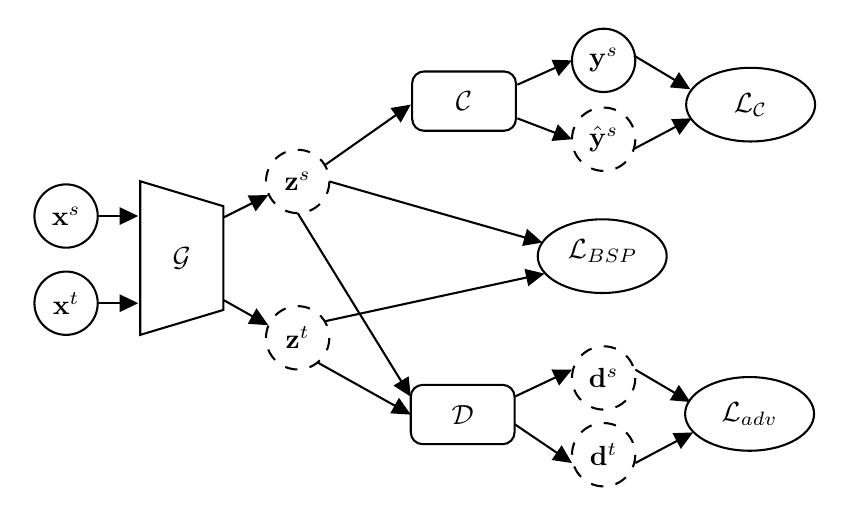
\begin{tikzpicture}[x=0.75pt,y=0.75pt,yscale=-1,xscale=1]
        %uncomment if require: \path (0,300); %set diagram left start at 0, and has height of 300

        %Shape: Circle [id:dp14395415737572304] 
        \draw   (57,126.75) .. controls (57,118.33) and (63.83,111.5) .. (72.25,111.5) .. controls (80.67,111.5) and (87.5,118.33) .. (87.5,126.75) .. controls (87.5,135.17) and (80.67,142) .. (72.25,142) .. controls (63.83,142) and (57,135.17) .. (57,126.75) -- cycle ;

        %Shape: Circle [id:dp5294927781460403] 
        \draw   (57,168.75) .. controls (57,160.33) and (63.83,153.5) .. (72.25,153.5) .. controls (80.67,153.5) and (87.5,160.33) .. (87.5,168.75) .. controls (87.5,177.17) and (80.67,184) .. (72.25,184) .. controls (63.83,184) and (57,177.17) .. (57,168.75) -- cycle ;

        %Shape: Trapezoid [id:dp3621515034386269] 
        \draw   (108,110) -- (148,122) -- (148,172) -- (108,184) -- cycle ;

        %Straight Lines [id:da711615291035981] 
        \draw    (87.5,126.75) -- (104,126.75) ;
        \draw [shift={(107,126.75)}, rotate = 180] [fill={rgb, 255:red, 0; green, 0; blue, 0 }  ][line width=0.08]  [draw opacity=0] (8.93,-4.29) -- (0,0) -- (8.93,4.29) -- cycle    ;
        %Shape: Circle [id:dp5854711906138592] 
        \draw  [dash pattern={on 4.5pt off 4.5pt}] (168.58,110.08) .. controls (168.58,101.66) and (175.41,94.83) .. (183.83,94.83) .. controls (192.26,94.83) and (199.08,101.66) .. (199.08,110.08) .. controls (199.08,118.51) and (192.26,125.33) .. (183.83,125.33) .. controls (175.41,125.33) and (168.58,118.51) .. (168.58,110.08) -- cycle ;

        %Shape: Circle [id:dp8402316163188099] 
        \draw  [dash pattern={on 4.5pt off 4.5pt}] (168.58,185.42) .. controls (168.58,176.99) and (175.41,170.17) .. (183.83,170.17) .. controls (192.26,170.17) and (199.08,176.99) .. (199.08,185.42) .. controls (199.08,193.84) and (192.26,200.67) .. (183.83,200.67) .. controls (175.41,200.67) and (168.58,193.84) .. (168.58,185.42) -- cycle ;

        %Rounded Rect [id:dp15165955457538138] 
        \draw   (239,62.81) .. controls (239,59.65) and (241.56,57.1) .. (244.71,57.1) -- (283.29,57.1) .. controls (286.44,57.1) and (289,59.65) .. (289,62.81) -- (289,79.95) .. controls (289,83.11) and (286.44,85.67) .. (283.29,85.67) -- (244.71,85.67) .. controls (241.56,85.67) and (239,83.11) .. (239,79.95) -- cycle ;

        %Rounded Rect [id:dp47289041628378614] 
        \draw   (238.33,213.81) .. controls (238.33,210.65) and (240.89,208.1) .. (244.05,208.1) -- (282.62,208.1) .. controls (285.77,208.1) and (288.33,210.65) .. (288.33,213.81) -- (288.33,230.95) .. controls (288.33,234.11) and (285.77,236.67) .. (282.62,236.67) -- (244.05,236.67) .. controls (240.89,236.67) and (238.33,234.11) .. (238.33,230.95) -- cycle ;

        %Shape: Circle [id:dp20484409800302994] 
        \draw  [dash pattern={on 4.5pt off 4.5pt}] (316,204.75) .. controls (316,196.33) and (322.83,189.5) .. (331.25,189.5) .. controls (339.67,189.5) and (346.5,196.33) .. (346.5,204.75) .. controls (346.5,213.17) and (339.67,220) .. (331.25,220) .. controls (322.83,220) and (316,213.17) .. (316,204.75) -- cycle ;

        %Shape: Circle [id:dp19954579063976796] 
        \draw  [dash pattern={on 4.5pt off 4.5pt}] (316,241.75) .. controls (316,233.33) and (322.83,226.5) .. (331.25,226.5) .. controls (339.67,226.5) and (346.5,233.33) .. (346.5,241.75) .. controls (346.5,250.17) and (339.67,257) .. (331.25,257) .. controls (322.83,257) and (316,250.17) .. (316,241.75) -- cycle ;

        %Shape: Ellipse [id:dp41632665310072503] 
        \draw   (370.5,222.08) .. controls (370.5,212.28) and (384.41,204.33) .. (401.56,204.33) .. controls (418.72,204.33) and (432.63,212.28) .. (432.63,222.08) .. controls (432.63,231.89) and (418.72,239.83) .. (401.56,239.83) .. controls (384.41,239.83) and (370.5,231.89) .. (370.5,222.08) -- cycle ;

        %Shape: Circle [id:dp17102829278099274] 
        \draw   (316,51.75) .. controls (316,43.33) and (322.83,36.5) .. (331.25,36.5) .. controls (339.67,36.5) and (346.5,43.33) .. (346.5,51.75) .. controls (346.5,60.17) and (339.67,67) .. (331.25,67) .. controls (322.83,67) and (316,60.17) .. (316,51.75) -- cycle ;
        %Shape: Circle [id:dp2918994940011912] 
        \draw  [dash pattern={on 4.5pt off 4.5pt}] (316,89.75) .. controls (316,81.33) and (322.83,74.5) .. (331.25,74.5) .. controls (339.67,74.5) and (346.5,81.33) .. (346.5,89.75) .. controls (346.5,98.17) and (339.67,105) .. (331.25,105) .. controls (322.83,105) and (316,98.17) .. (316,89.75) -- cycle ;
        %Shape: Ellipse [id:dp7208514036481783] 
        \draw   (371,73.08) .. controls (371,63.28) and (384.91,55.33) .. (402.06,55.33) .. controls (419.22,55.33) and (433.13,63.28) .. (433.13,73.08) .. controls (433.13,82.89) and (419.22,90.83) .. (402.06,90.83) .. controls (384.91,90.83) and (371,82.89) .. (371,73.08) -- cycle ;
        %Straight Lines [id:da35699780719749463] 
        \draw    (87.5,168.75) -- (104,168.75) ;
        \draw [shift={(107,168.75)}, rotate = 180] [fill={rgb, 255:red, 0; green, 0; blue, 0 }  ][line width=0.08]  [draw opacity=0] (8.93,-4.29) -- (0,0) -- (8.93,4.29) -- cycle    ;
        %Straight Lines [id:da18773339124658595] 
        \draw    (148.33,127.33) -- (166.98,118.01) ;
        \draw [shift={(169.67,116.67)}, rotate = 153.43] [fill={rgb, 255:red, 0; green, 0; blue, 0 }  ][line width=0.08]  [draw opacity=0] (8.93,-4.29) -- (0,0) -- (8.93,4.29) -- cycle    ;
        %Straight Lines [id:da22178069673434142] 
        \draw    (148.33,167.33) -- (167.05,177.86) ;
        \draw [shift={(169.67,179.33)}, rotate = 209.36] [fill={rgb, 255:red, 0; green, 0; blue, 0 }  ][line width=0.08]  [draw opacity=0] (8.93,-4.29) -- (0,0) -- (8.93,4.29) -- cycle    ;
        %Straight Lines [id:da7263329854343115] 
        \draw    (197.25,102) -- (235.88,74.81) ;
        \draw [shift={(238.33,73.08)}, rotate = 144.86] [fill={rgb, 255:red, 0; green, 0; blue, 0 }  ][line width=0.08]  [draw opacity=0] (8.93,-4.29) -- (0,0) -- (8.93,4.29) -- cycle    ;
        %Straight Lines [id:da5895896069004276] 
        \draw    (193.6,197.4) -- (235.71,220.95) ;
        \draw [shift={(238.33,222.42)}, rotate = 209.22] [fill={rgb, 255:red, 0; green, 0; blue, 0 }  ][line width=0.08]  [draw opacity=0] (8.93,-4.29) -- (0,0) -- (8.93,4.29) -- cycle    ;
        %Straight Lines [id:da504234275800213] 
        \draw    (183.83,125.33) -- (236.76,211.26) ;
        \draw [shift={(238.33,213.81)}, rotate = 238.37] [fill={rgb, 255:red, 0; green, 0; blue, 0 }  ][line width=0.08]  [draw opacity=0] (8.93,-4.29) -- (0,0) -- (8.93,4.29) -- cycle    ;
        %Straight Lines [id:da10127819240633107] 
        \draw    (288.33,213.81) -- (313.29,202.03) ;
        \draw [shift={(316,200.75)}, rotate = 154.73] [fill={rgb, 255:red, 0; green, 0; blue, 0 }  ][line width=0.08]  [draw opacity=0] (8.93,-4.29) -- (0,0) -- (8.93,4.29) -- cycle    ;
        %Straight Lines [id:da18118282714853473] 
        \draw    (288.33,227) -- (313.52,244.07) ;
        \draw [shift={(316,245.75)}, rotate = 214.13] [fill={rgb, 255:red, 0; green, 0; blue, 0 }  ][line width=0.08]  [draw opacity=0] (8.93,-4.29) -- (0,0) -- (8.93,4.29) -- cycle    ;
        %Straight Lines [id:da46435990995985477] 
        \draw    (346.5,200.75) -- (370.41,214.81) ;
        \draw [shift={(373,216.33)}, rotate = 210.46] [fill={rgb, 255:red, 0; green, 0; blue, 0 }  ][line width=0.08]  [draw opacity=0] (8.93,-4.29) -- (0,0) -- (8.93,4.29) -- cycle    ;
        %Straight Lines [id:da3066500527802958] 
        \draw    (346.5,245.75) -- (371.68,232.4) ;
        \draw [shift={(374.33,231)}, rotate = 152.08] [fill={rgb, 255:red, 0; green, 0; blue, 0 }  ][line width=0.08]  [draw opacity=0] (8.93,-4.29) -- (0,0) -- (8.93,4.29) -- cycle    ;
        %Straight Lines [id:da9357957653419868] 
        \draw    (289.67,63.48) -- (313.26,52.97) ;
        \draw [shift={(316,51.75)}, rotate = 156] [fill={rgb, 255:red, 0; green, 0; blue, 0 }  ][line width=0.08]  [draw opacity=0] (8.93,-4.29) -- (0,0) -- (8.93,4.29) -- cycle    ;
        %Straight Lines [id:da5822336916421971] 
        \draw    (289.67,79.67) -- (313.2,88.68) ;
        \draw [shift={(316,89.75)}, rotate = 200.95] [fill={rgb, 255:red, 0; green, 0; blue, 0 }  ][line width=0.08]  [draw opacity=0] (8.93,-4.29) -- (0,0) -- (8.93,4.29) -- cycle    ;
        %Straight Lines [id:da8400721166176619] 
        \draw    (345.83,49.42) -- (370.43,64.13) ;
        \draw [shift={(373,65.67)}, rotate = 210.89] [fill={rgb, 255:red, 0; green, 0; blue, 0 }  ][line width=0.08]  [draw opacity=0] (8.93,-4.29) -- (0,0) -- (8.93,4.29) -- cycle    ;
        %Straight Lines [id:da5048948243554285] 
        \draw    (345.83,94.42) -- (371.02,81.07) ;
        \draw [shift={(373.67,79.67)}, rotate = 152.08] [fill={rgb, 255:red, 0; green, 0; blue, 0 }  ][line width=0.08]  [draw opacity=0] (8.93,-4.29) -- (0,0) -- (8.93,4.29) -- cycle    ;
        %Shape: Ellipse [id:dp8464659325338855] 
        \draw   (299.5,146.08) .. controls (299.5,136.28) and (313.41,128.33) .. (330.56,128.33) .. controls (347.72,128.33) and (361.63,136.28) .. (361.63,146.08) .. controls (361.63,155.89) and (347.72,163.83) .. (330.56,163.83) .. controls (313.41,163.83) and (299.5,155.89) .. (299.5,146.08) -- cycle ;
        %Straight Lines [id:da5523565128759309] 
        \draw    (197.2,177.4) -- (299.82,155.14) ;
        \draw [shift={(302.75,154.5)}, rotate = 167.76] [fill={rgb, 255:red, 0; green, 0; blue, 0 }  ][line width=0.08]  [draw opacity=0] (8.93,-4.29) -- (0,0) -- (8.93,4.29) -- cycle    ;
        %Straight Lines [id:da24838256047555873] 
        \draw    (199.08,110.08) -- (298.87,138.67) ;
        \draw [shift={(301.75,139.5)}, rotate = 195.99] [fill={rgb, 255:red, 0; green, 0; blue, 0 }  ][line width=0.08]  [draw opacity=0] (8.93,-4.29) -- (0,0) -- (8.93,4.29) -- cycle    ;

        % Text Node
        \draw (331.25,51.75) node   [align=left] {\begin{minipage}[lt]{21.08pt}\setlength\topsep{0pt}
                \begin{center}
                    $\mathbf{y}^s$
                \end{center}

            \end{minipage}};
        % Text Node
        \draw (331.25,89.75) node   [align=left] {\begin{minipage}[lt]{21.08pt}\setlength\topsep{0pt}
                \begin{center}
                    $\hat{\mathbf{y}}^s$
                \end{center}

            \end{minipage}};
        % Text Node
        \draw (402.06,73.08) node   [align=left] {\begin{minipage}[lt]{32.64pt}\setlength\topsep{0pt}
                \begin{center}
                    $\mathcal{L}_{\mathcal{C}}$
                \end{center}

            \end{minipage}};
        % Text Node
        \draw (401.56,222.08) node   [align=left] {\begin{minipage}[lt]{32.64pt}\setlength\topsep{0pt}
                \begin{center}
                    $\mathcal{L}_{adv}$
                \end{center}

            \end{minipage}};
        % Text Node
        \draw (331.25,241.75) node   [align=left] {\begin{minipage}[lt]{21.08pt}\setlength\topsep{0pt}
                \begin{center}
                    $\mathbf{d}^t$
                \end{center}

            \end{minipage}};
        % Text Node
        \draw (331.25,204.75) node   [align=left] {\begin{minipage}[lt]{21.08pt}\setlength\topsep{0pt}
                \begin{center}
                    $\mathbf{d}^s$
                \end{center}

            \end{minipage}};
        % Text Node
        \draw (263.33,222.56) node   [align=left] {\begin{minipage}[lt]{26.23pt}\setlength\topsep{0pt}
                \begin{center}
                    $\mathcal{D}$
                \end{center}

            \end{minipage}};
        % Text Node
        \draw (264,71.56) node   [align=left] {\begin{minipage}[lt]{26.23pt}\setlength\topsep{0pt}
                \begin{center}
                    $\mathcal{C}$
                \end{center}

            \end{minipage}};
        % Text Node
        \draw (183.83,185.42) node   [align=left] {\begin{minipage}[lt]{21.08pt}\setlength\topsep{0pt}
                \begin{center}
                    $\mathbf{z}^t$
                \end{center}

            \end{minipage}};
        % Text Node
        \draw (183.83,110.08) node   [align=left] {\begin{minipage}[lt]{21.08pt}\setlength\topsep{0pt}
                \begin{center}
                    $\mathbf{z}^s$
                \end{center}

            \end{minipage}};
        % Text Node
        \draw (128,147) node   [align=left] {\begin{minipage}[lt]{22.78pt}\setlength\topsep{0pt}
                \begin{center}
                    $\mathcal{G}$
                \end{center}

            \end{minipage}};
        % Text Node
        \draw (72.25,168.75) node   [align=left] {\begin{minipage}[lt]{21.08pt}\setlength\topsep{0pt}
                \begin{center}
                    $\mathbf{x}^t$
                \end{center}

            \end{minipage}};
        % Text Node
        \draw (72.25,126.75) node   [align=left] {\begin{minipage}[lt]{21.08pt}\setlength\topsep{0pt}
                \begin{center}
                    $\mathbf{x}^s$
                \end{center}

            \end{minipage}};
        % Text Node
        \draw (312.5,136.4) node [anchor=north west][inner sep=0.75pt]    {$\mathcal{L}_{BSP} $};

    \end{tikzpicture}

    \caption{Esquema de un modelo {\it DANN+BSP}.}
    \label{fig:bsp-esquema-dann}
\end{figure}

Por lo tanto, un modelo {\it DANN+BSP} presenta como objetivos:

\begin{align}
     & \min_{\mathcal{G},\mathcal{C}} \mathcal{L}_\mathcal{C}(\mathbf{x}^s, \mathbf{y}^s) + \lambda \mathcal{L}_{adv}(\mathbf{x}^s, \mathbf{x}^t) + \beta \mathcal{L}_{BSP}(\mathcal{G}(\mathbf{x})) \\
     & \max_{\mathcal{D}} \mathcal{L}_{adv}(\mathbf{x}^s, \mathbf{x}^t)
    \label{eq:bsp-dann-obejtivo}
\end{align}

Donde $\beta$ es el par\'ametro que regula el trade-off de $\mathcal{L}_{BSP}$.

\subsection{Margin Disparity Discrepancy}

Las t\'ecnicas detalladas hasta el momento implican algoritmos de optimizaci\'on minimax, que funcionan correctamente
en los m\'etodos basados en el aprendizaje adversario. Sin embargo, estos algoritmos utilizan funciones de scoreoque
carecen de garant\'ias te\'oricas ya que se estudiaron funciones de p\'erdida 0-1. Es por esto que se introducen
m\'etodos que apuntan a reducir la brecha que existe entre la teor\'ia y el algoritmo, como Margin Disparity
Discrepancy {\it MDD} \parencite{zhang2019bridging}.

\begin{figure}[H]
    \centering

    \tikzset{every picture/.style={line width=0.75pt}} %set default line width to 0.75pt        

    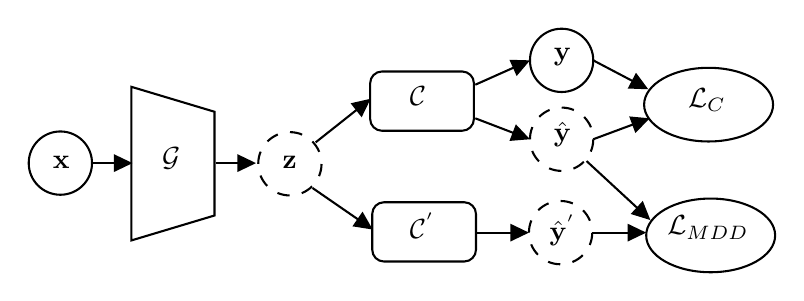
\begin{tikzpicture}[x=0.75pt,y=0.75pt,yscale=-1,xscale=1]
        %uncomment if require: \path (0,424); %set diagram left start at 0, and has height of 424

        %Shape: Circle [id:dp37402229817841603] 
        \draw   (60.5,104.75) .. controls (60.5,96.33) and (67.33,89.5) .. (75.75,89.5) .. controls (84.17,89.5) and (91,96.33) .. (91,104.75) .. controls (91,113.17) and (84.17,120) .. (75.75,120) .. controls (67.33,120) and (60.5,113.17) .. (60.5,104.75) -- cycle ;
        %Shape: Trapezoid [id:dp5518581764728496] 
        \draw   (110,68) -- (150,80) -- (150,130) -- (110,142) -- cycle ;
        %Straight Lines [id:da7900111351501842] 
        \draw    (91,104.75) -- (107.5,104.75) ;
        \draw [shift={(110.5,104.75)}, rotate = 180] [fill={rgb, 255:red, 0; green, 0; blue, 0 }  ][line width=0.08]  [draw opacity=0] (8.93,-4.29) -- (0,0) -- (8.93,4.29) -- cycle    ;
        %Shape: Circle [id:dp6237032464701955] 
        \draw  [dash pattern={on 4.5pt off 4.5pt}] (171.08,105.08) .. controls (171.08,96.66) and (177.91,89.83) .. (186.33,89.83) .. controls (194.76,89.83) and (201.58,96.66) .. (201.58,105.08) .. controls (201.58,113.51) and (194.76,120.33) .. (186.33,120.33) .. controls (177.91,120.33) and (171.08,113.51) .. (171.08,105.08) -- cycle ;
        %Rounded Rect [id:dp17455651105714143] 
        \draw   (225,66.31) .. controls (225,63.15) and (227.56,60.6) .. (230.71,60.6) -- (269.29,60.6) .. controls (272.44,60.6) and (275,63.15) .. (275,66.31) -- (275,83.45) .. controls (275,86.61) and (272.44,89.17) .. (269.29,89.17) -- (230.71,89.17) .. controls (227.56,89.17) and (225,86.61) .. (225,83.45) -- cycle ;
        %Shape: Circle [id:dp2140151642409336] 
        \draw   (302,55.25) .. controls (302,46.83) and (308.83,40) .. (317.25,40) .. controls (325.67,40) and (332.5,46.83) .. (332.5,55.25) .. controls (332.5,63.67) and (325.67,70.5) .. (317.25,70.5) .. controls (308.83,70.5) and (302,63.67) .. (302,55.25) -- cycle ;
        %Shape: Circle [id:dp8313620493224034] 
        \draw  [dash pattern={on 4.5pt off 4.5pt}] (302,93.25) .. controls (302,84.83) and (308.83,78) .. (317.25,78) .. controls (325.67,78) and (332.5,84.83) .. (332.5,93.25) .. controls (332.5,101.67) and (325.67,108.5) .. (317.25,108.5) .. controls (308.83,108.5) and (302,101.67) .. (302,93.25) -- cycle ;
        %Shape: Ellipse [id:dp0600451143745524] 
        \draw   (357,76.58) .. controls (357,66.78) and (370.91,58.83) .. (388.06,58.83) .. controls (405.22,58.83) and (419.13,66.78) .. (419.13,76.58) .. controls (419.13,86.39) and (405.22,94.33) .. (388.06,94.33) .. controls (370.91,94.33) and (357,86.39) .. (357,76.58) -- cycle ;
        %Straight Lines [id:da9980456278456524] 
        \draw    (198.75,94.75) -- (222.9,75.61) ;
        \draw [shift={(225.25,73.75)}, rotate = 141.6] [fill={rgb, 255:red, 0; green, 0; blue, 0 }  ][line width=0.08]  [draw opacity=0] (8.93,-4.29) -- (0,0) -- (8.93,4.29) -- cycle    ;
        %Straight Lines [id:da3629940013678272] 
        \draw    (275.67,66.98) -- (299.26,56.47) ;
        \draw [shift={(302,55.25)}, rotate = 156] [fill={rgb, 255:red, 0; green, 0; blue, 0 }  ][line width=0.08]  [draw opacity=0] (8.93,-4.29) -- (0,0) -- (8.93,4.29) -- cycle    ;
        %Straight Lines [id:da8352907095901936] 
        \draw    (275.67,83.17) -- (299.2,92.18) ;
        \draw [shift={(302,93.25)}, rotate = 200.95] [fill={rgb, 255:red, 0; green, 0; blue, 0 }  ][line width=0.08]  [draw opacity=0] (8.93,-4.29) -- (0,0) -- (8.93,4.29) -- cycle    ;
        %Straight Lines [id:da1138581727231831] 
        \draw    (332.5,55.25) -- (356.34,67.77) ;
        \draw [shift={(359,69.17)}, rotate = 207.71] [fill={rgb, 255:red, 0; green, 0; blue, 0 }  ][line width=0.08]  [draw opacity=0] (8.93,-4.29) -- (0,0) -- (8.93,4.29) -- cycle    ;
        %Straight Lines [id:da07484994635417963] 
        \draw    (332.5,93.25) -- (356.85,84.21) ;
        \draw [shift={(359.67,83.17)}, rotate = 159.64] [fill={rgb, 255:red, 0; green, 0; blue, 0 }  ][line width=0.08]  [draw opacity=0] (8.93,-4.29) -- (0,0) -- (8.93,4.29) -- cycle    ;
        %Straight Lines [id:da7386987904124067] 
        \draw    (150.5,104.75) -- (167,104.75) ;
        \draw [shift={(170,104.75)}, rotate = 180] [fill={rgb, 255:red, 0; green, 0; blue, 0 }  ][line width=0.08]  [draw opacity=0] (8.93,-4.29) -- (0,0) -- (8.93,4.29) -- cycle    ;
        %Rounded Rect [id:dp7058372380502067] 
        \draw   (226,129.31) .. controls (226,126.15) and (228.56,123.6) .. (231.71,123.6) -- (270.29,123.6) .. controls (273.44,123.6) and (276,126.15) .. (276,129.31) -- (276,146.45) .. controls (276,149.61) and (273.44,152.17) .. (270.29,152.17) -- (231.71,152.17) .. controls (228.56,152.17) and (226,149.61) .. (226,146.45) -- cycle ;
        %Shape: Circle [id:dp8799954567091415] 
        \draw  [dash pattern={on 4.5pt off 4.5pt}] (301.5,138.25) .. controls (301.5,129.83) and (308.33,123) .. (316.75,123) .. controls (325.17,123) and (332,129.83) .. (332,138.25) .. controls (332,146.67) and (325.17,153.5) .. (316.75,153.5) .. controls (308.33,153.5) and (301.5,146.67) .. (301.5,138.25) -- cycle ;
        %Shape: Ellipse [id:dp09534345336772221] 
        \draw   (358,139.58) .. controls (358,129.78) and (371.91,121.83) .. (389.06,121.83) .. controls (406.22,121.83) and (420.13,129.78) .. (420.13,139.58) .. controls (420.13,149.39) and (406.22,157.33) .. (389.06,157.33) .. controls (371.91,157.33) and (358,149.39) .. (358,139.58) -- cycle ;
        %Straight Lines [id:da6601974145410334] 
        \draw    (197.25,116.75) -- (223.78,135.05) ;
        \draw [shift={(226.25,136.75)}, rotate = 214.59] [fill={rgb, 255:red, 0; green, 0; blue, 0 }  ][line width=0.08]  [draw opacity=0] (8.93,-4.29) -- (0,0) -- (8.93,4.29) -- cycle    ;
        %Straight Lines [id:da32804094797701633] 
        \draw    (275.75,138.25) -- (298.5,138.25) ;
        \draw [shift={(301.5,138.25)}, rotate = 180] [fill={rgb, 255:red, 0; green, 0; blue, 0 }  ][line width=0.08]  [draw opacity=0] (8.93,-4.29) -- (0,0) -- (8.93,4.29) -- cycle    ;
        %Straight Lines [id:da19377630354971975] 
        \draw    (329.25,103.75) -- (357.8,130.13) ;
        \draw [shift={(360,132.17)}, rotate = 222.74] [fill={rgb, 255:red, 0; green, 0; blue, 0 }  ][line width=0.08]  [draw opacity=0] (8.93,-4.29) -- (0,0) -- (8.93,4.29) -- cycle    ;
        %Straight Lines [id:da39400351361192065] 
        \draw    (332,138.25) -- (355,138.25) ;
        \draw [shift={(358,138.25)}, rotate = 180] [fill={rgb, 255:red, 0; green, 0; blue, 0 }  ][line width=0.08]  [draw opacity=0] (8.93,-4.29) -- (0,0) -- (8.93,4.29) -- cycle    ;

        % Text Node
        \draw (70.67,100) node [anchor=north west][inner sep=0.75pt]    {$\mathbf{x}$};
        % Text Node
        \draw (123.33,95.73) node [anchor=north west][inner sep=0.75pt]    {$\mathcal{G}$};
        % Text Node
        \draw (181.33,100) node [anchor=north west][inner sep=0.75pt]    {$\mathbf{z}$};
        % Text Node
        \draw (242.67,66.4) node [anchor=north west][inner sep=0.75pt]    {$\mathcal{C}$};
        % Text Node
        \draw (242.67,127) node [anchor=north west][inner sep=0.75pt]    {$\mathcal{C}^{'}$};
        % Text Node
        \draw (310,128) node [anchor=north west][inner sep=0.75pt]    {$\hat{\mathbf{y}}^{'}$};
        % Text Node
        \draw (312,83.4) node [anchor=north west][inner sep=0.75pt]    {$\hat{\mathbf{y}}$};
        % Text Node
        \draw (312,48) node [anchor=north west][inner sep=0.75pt]    {$\mathbf{y}$};
        % Text Node
        \draw (376.67,67.4) node [anchor=north west][inner sep=0.75pt]    {$\mathcal{L}_{C}$};
        % Text Node
        \draw (366.67,128.73) node [anchor=north west][inner sep=0.75pt]    {$\mathcal{L}_{MDD}$};

    \end{tikzpicture}
    \caption{Esquema de {\it MDD}. Los c\'irculos con l\'ineas rayadas son salidas de los modelos mientras que los c\'irculos de l\'ineas s\'olidas son datos conocidos.
            {\it MDD} introduce un clasificador clasificador adversario $\mathcal{C}^{'}$ para maximizar la discrepancia y entrena el generador de características $\mathcal{G}$ para
        minimizar el error de origen como tambien la discrepancia.}
    \label{fig:mdd-esquema}
\end{figure}

$\mathcal{L}_{\mathcal{C}}$ contin\'ua siendo la funci\'on {\it cross-entropy} $\mathcal{L}_{CE}$ aplicado a la salida de la red $\mathcal{C}$.

\begin{align}
    \min_{\mathcal{C}} \mathcal{L}_\mathcal{C}(\mathbf{x}^s, \mathbf{y}^s) = \mathcal{L}_{CE}(C(\mathcal{G}(\mathbf{x}^s)), \mathbf{y}^s)
    \label{eq:mdd-loss-clasificadora}
\end{align}

Por otro lado, $\mathcal{L}_{\mathcal{MDD}}$ contiene un {\it margen} $\rho$ que se obtiene introduciendo el
par\'ametro $\gamma \triangleq \exp \rho$ en la ecuaci\'on \ref{eq:mdd-loss}.

\begin{align}
    \max_{\mathcal{C}^{'}} \mathcal{L}_{\mathcal{MDD}}(\mathbf{x}^s, \mathbf{x}^t) = & \gamma \mathbb{E}_{\mathbf{x}^s \sim \mathcal{\hat{S}}} \log[\sigma(\mathcal{C}^{'}(\mathcal{G}(\mathbf{x}^s)))] + \nonumber \\
                                                                                     & \mathbb{E}_{\mathbf{x}^t \sim \mathcal{\hat{T}}} \log[1-\sigma(\mathcal{C}^{'}(\mathcal{G}(\mathbf{x}^t)))]
    \label{eq:mdd-loss}
\end{align}

Donde $\sigma$ es la funci\'on {\it softmax}. Por lo tanto, el objetivo de optimización viene dado por la ecuaci\'on
\ref{eq:mdd-objetivo}, donde $\lambda$ es el trade-off entre la clasificaci\'on y la discriminaci\'on adversaria.

\begin{align}
    \min_{\mathcal{G}, \mathcal{C}} \mathcal{L}_{\mathcal{C}}(\mathbf{x}^s, \mathbf{x}^t) + \lambda \mathcal{L}_{\mathcal{MDD}}(\mathbf{x}^s, \mathbf{x}^t)
    \label{eq:mdd-objetivo}
\end{align}

\subsection{Adaptive Feature Norm}

El mayor problema que surge de la adaptaci\'on de dominio es la degradaci\'on del modelo en cuanto a la clasificaci\'on \parencite{yosinski2014transferable}. Las divergencias estadísticas existentes pueden no representar con precisión el
cambio de dominio y subsanar tales discrepancias puede no garantizar la transferencia entre dominios. Tales
discrepancias se ejemplifican en la figura \ref{fig:afn-source-only}.

\begin{figure}[H]
    \centering
    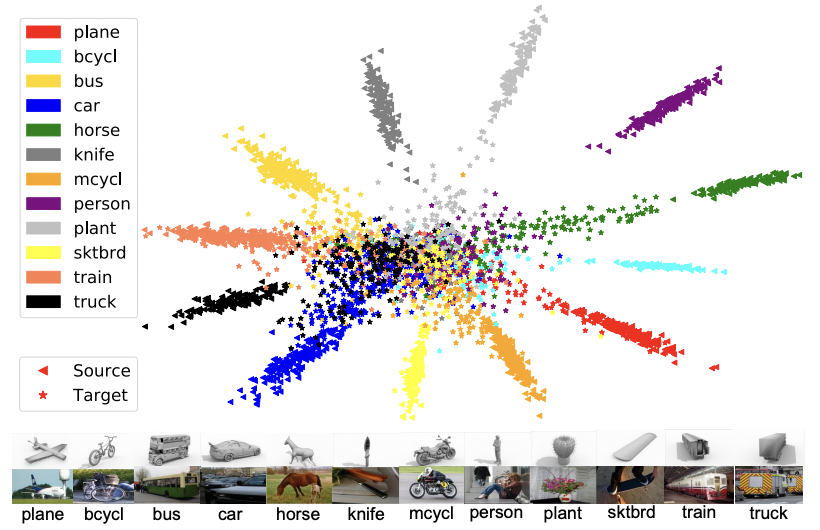
\includegraphics[width=0.7\textwidth]{chapter2/afn-visda-source-only.png}

    \caption{Visualizaci\'on de las características aprendidas para el origen y destino utilizando un modelo entrenado utilizando muestras del origen. Imagen tomada de \cite{xu2019larger}.}
    \label{fig:afn-source-only}
\end{figure}

Esto sugiere que las normas excesivamente pequeñas de las muestras de destino con respecto a las de origen explican el
deterioro en la clasificación. No obstante, pueden plantearse dos hipótesis:

\begin{itemize}
    \item Normas de las características desalineadas: el desplazamiento entre los dominios de origen y destino se explica en la
          desalineación de los valores esperados de las normas de sus características. La coincidencia de las normas de ambos
          dominios a un escalar arbitrariamente elegido supondrá una mejora en la transferencias.
    \item Norma de las caracteristicas más pequeña: el desplazamiento entre los dominios se explica debido a las características
          menos informativas con normas más pequeñas del dominio de destino. Adaptar las características de destino a regiones
          alejadas de las normas pequeñas supondrá una mejora en la transferencia.
\end{itemize}

\cite{xu2019larger} propone un método llamado {\it Adaptive Feature Norm AFN} que consiste en normalizar las normas de las características aprendidas por la red $\mathcal{G}$  mediante $n$ bloques $\mathcal{N}$ (compuestos por FC-BN-ReLU-Dropout) y mediante $\mathcal{L}_{AFN}$.

\begin{figure}[H]
    \centering

    \tikzset{every picture/.style={line width=0.75pt}} %set default line width to 0.75pt        

    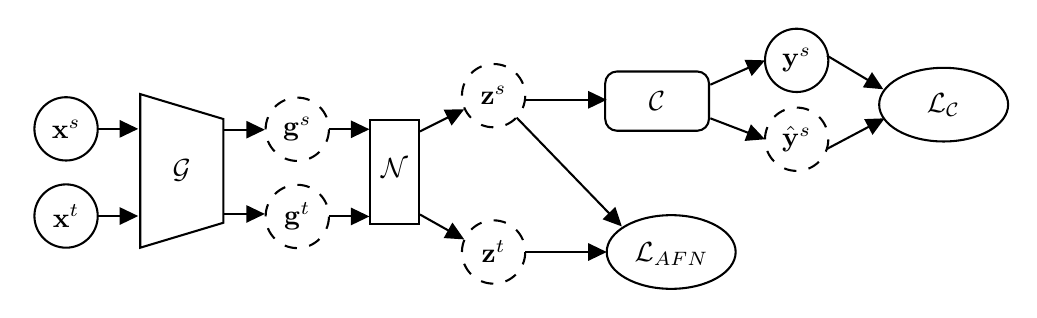
\begin{tikzpicture}[x=0.75pt,y=0.75pt,yscale=-1,xscale=1]
        %uncomment if require: \path (0,409); %set diagram left start at 0, and has height of 409

        %Shape: Circle [id:dp36883064074545446] 
        \draw   (59,84.75) .. controls (59,76.33) and (65.83,69.5) .. (74.25,69.5) .. controls (82.67,69.5) and (89.5,76.33) .. (89.5,84.75) .. controls (89.5,93.17) and (82.67,100) .. (74.25,100) .. controls (65.83,100) and (59,93.17) .. (59,84.75) -- cycle ;

        %Shape: Circle [id:dp7170555789489086] 
        \draw   (59,126.75) .. controls (59,118.33) and (65.83,111.5) .. (74.25,111.5) .. controls (82.67,111.5) and (89.5,118.33) .. (89.5,126.75) .. controls (89.5,135.17) and (82.67,142) .. (74.25,142) .. controls (65.83,142) and (59,135.17) .. (59,126.75) -- cycle ;

        %Shape: Trapezoid [id:dp6591706550778527] 
        \draw   (110,68) -- (150,80) -- (150,130) -- (110,142) -- cycle ;

        %Straight Lines [id:da8866180371172607] 
        \draw    (89.5,84.75) -- (106,84.75) ;
        \draw [shift={(109,84.75)}, rotate = 180] [fill={rgb, 255:red, 0; green, 0; blue, 0 }  ][line width=0.08]  [draw opacity=0] (8.93,-4.29) -- (0,0) -- (8.93,4.29) -- cycle    ;
        %Shape: Circle [id:dp7226735192986846] 
        \draw  [dash pattern={on 4.5pt off 4.5pt}] (264.98,68.75) .. controls (264.98,60.33) and (271.81,53.5) .. (280.23,53.5) .. controls (288.66,53.5) and (295.48,60.33) .. (295.48,68.75) .. controls (295.48,77.17) and (288.66,84) .. (280.23,84) .. controls (271.81,84) and (264.98,77.17) .. (264.98,68.75) -- cycle ;
        %Shape: Circle [id:dp11338914726883309] 
        \draw  [dash pattern={on 4.5pt off 4.5pt}] (264.98,144.08) .. controls (264.98,135.66) and (271.81,128.83) .. (280.23,128.83) .. controls (288.66,128.83) and (295.48,135.66) .. (295.48,144.08) .. controls (295.48,152.51) and (288.66,159.33) .. (280.23,159.33) .. controls (271.81,159.33) and (264.98,152.51) .. (264.98,144.08) -- cycle ;
        %Straight Lines [id:da7817124779055846] 
        \draw    (89.5,126.75) -- (106,126.75) ;
        \draw [shift={(109,126.75)}, rotate = 180] [fill={rgb, 255:red, 0; green, 0; blue, 0 }  ][line width=0.08]  [draw opacity=0] (8.93,-4.29) -- (0,0) -- (8.93,4.29) -- cycle    ;
        %Straight Lines [id:da7526972599979318] 
        \draw    (244.73,86) -- (263.38,76.67) ;
        \draw [shift={(266.07,75.33)}, rotate = 153.43] [fill={rgb, 255:red, 0; green, 0; blue, 0 }  ][line width=0.08]  [draw opacity=0] (8.93,-4.29) -- (0,0) -- (8.93,4.29) -- cycle    ;
        %Straight Lines [id:da13505401193908728] 
        \draw    (244.73,126) -- (263.45,136.53) ;
        \draw [shift={(266.07,138)}, rotate = 209.36] [fill={rgb, 255:red, 0; green, 0; blue, 0 }  ][line width=0.08]  [draw opacity=0] (8.93,-4.29) -- (0,0) -- (8.93,4.29) -- cycle    ;
        %Straight Lines [id:da4909359959704669] 
        \draw    (295.48,70.75) -- (331.73,70.75) ;
        \draw [shift={(334.73,70.75)}, rotate = 180] [fill={rgb, 255:red, 0; green, 0; blue, 0 }  ][line width=0.08]  [draw opacity=0] (8.93,-4.29) -- (0,0) -- (8.93,4.29) -- cycle    ;
        %Straight Lines [id:da25373400738229757] 
        \draw    (295.48,144.08) -- (331.73,144.08) ;
        \draw [shift={(334.73,144.08)}, rotate = 180] [fill={rgb, 255:red, 0; green, 0; blue, 0 }  ][line width=0.08]  [draw opacity=0] (8.93,-4.29) -- (0,0) -- (8.93,4.29) -- cycle    ;
        %Shape: Rectangle [id:dp03201668448552586] 
        \draw   (220.67,80.6) -- (244.33,80.6) -- (244.33,130.4) -- (220.67,130.4) -- cycle ;

        %Shape: Circle [id:dp0590517882755186] 
        \draw  [dash pattern={on 4.5pt off 4.5pt}] (170.4,84.95) .. controls (170.4,76.53) and (177.23,69.7) .. (185.65,69.7) .. controls (194.07,69.7) and (200.9,76.53) .. (200.9,84.95) .. controls (200.9,93.37) and (194.07,100.2) .. (185.65,100.2) .. controls (177.23,100.2) and (170.4,93.37) .. (170.4,84.95) -- cycle ;
        %Shape: Circle [id:dp9792876246953977] 
        \draw  [dash pattern={on 4.5pt off 4.5pt}] (170.4,126.95) .. controls (170.4,118.53) and (177.23,111.7) .. (185.65,111.7) .. controls (194.07,111.7) and (200.9,118.53) .. (200.9,126.95) .. controls (200.9,135.37) and (194.07,142.2) .. (185.65,142.2) .. controls (177.23,142.2) and (170.4,135.37) .. (170.4,126.95) -- cycle ;
        %Straight Lines [id:da9352682997505948] 
        \draw    (200.9,84.95) -- (217.4,84.95) ;
        \draw [shift={(220.4,84.95)}, rotate = 180] [fill={rgb, 255:red, 0; green, 0; blue, 0 }  ][line width=0.08]  [draw opacity=0] (8.93,-4.29) -- (0,0) -- (8.93,4.29) -- cycle    ;
        %Straight Lines [id:da9288909607910223] 
        \draw    (200.9,126.95) -- (217.4,126.95) ;
        \draw [shift={(220.4,126.95)}, rotate = 180] [fill={rgb, 255:red, 0; green, 0; blue, 0 }  ][line width=0.08]  [draw opacity=0] (8.93,-4.29) -- (0,0) -- (8.93,4.29) -- cycle    ;
        %Straight Lines [id:da42477525756570467] 
        \draw    (150.5,85.15) -- (167,85.15) ;
        \draw [shift={(170,85.15)}, rotate = 180] [fill={rgb, 255:red, 0; green, 0; blue, 0 }  ][line width=0.08]  [draw opacity=0] (8.93,-4.29) -- (0,0) -- (8.93,4.29) -- cycle    ;
        %Straight Lines [id:da19510792007996902] 
        \draw    (150.5,125.75) -- (167,125.75) ;
        \draw [shift={(170,125.75)}, rotate = 180] [fill={rgb, 255:red, 0; green, 0; blue, 0 }  ][line width=0.08]  [draw opacity=0] (8.93,-4.29) -- (0,0) -- (8.93,4.29) -- cycle    ;
        %Rounded Rect [id:dp8233373593250533] 
        \draw   (334,62.81) .. controls (334,59.65) and (336.56,57.1) .. (339.71,57.1) -- (378.29,57.1) .. controls (381.44,57.1) and (384,59.65) .. (384,62.81) -- (384,79.95) .. controls (384,83.11) and (381.44,85.67) .. (378.29,85.67) -- (339.71,85.67) .. controls (336.56,85.67) and (334,83.11) .. (334,79.95) -- cycle ;

        %Shape: Circle [id:dp361141070335256] 
        \draw   (411,51.75) .. controls (411,43.33) and (417.83,36.5) .. (426.25,36.5) .. controls (434.67,36.5) and (441.5,43.33) .. (441.5,51.75) .. controls (441.5,60.17) and (434.67,67) .. (426.25,67) .. controls (417.83,67) and (411,60.17) .. (411,51.75) -- cycle ;
        %Shape: Circle [id:dp994981759860698] 
        \draw  [dash pattern={on 4.5pt off 4.5pt}] (411,89.75) .. controls (411,81.33) and (417.83,74.5) .. (426.25,74.5) .. controls (434.67,74.5) and (441.5,81.33) .. (441.5,89.75) .. controls (441.5,98.17) and (434.67,105) .. (426.25,105) .. controls (417.83,105) and (411,98.17) .. (411,89.75) -- cycle ;
        %Shape: Ellipse [id:dp4863694749188221] 
        \draw   (466,73.08) .. controls (466,63.28) and (479.91,55.33) .. (497.06,55.33) .. controls (514.22,55.33) and (528.13,63.28) .. (528.13,73.08) .. controls (528.13,82.89) and (514.22,90.83) .. (497.06,90.83) .. controls (479.91,90.83) and (466,82.89) .. (466,73.08) -- cycle ;
        %Straight Lines [id:da7034112467211542] 
        \draw    (384.67,63.48) -- (408.26,52.97) ;
        \draw [shift={(411,51.75)}, rotate = 156] [fill={rgb, 255:red, 0; green, 0; blue, 0 }  ][line width=0.08]  [draw opacity=0] (8.93,-4.29) -- (0,0) -- (8.93,4.29) -- cycle    ;
        %Straight Lines [id:da28235679904283506] 
        \draw    (384.67,79.67) -- (408.2,88.68) ;
        \draw [shift={(411,89.75)}, rotate = 200.95] [fill={rgb, 255:red, 0; green, 0; blue, 0 }  ][line width=0.08]  [draw opacity=0] (8.93,-4.29) -- (0,0) -- (8.93,4.29) -- cycle    ;
        %Straight Lines [id:da3443605473479898] 
        \draw    (440.83,49.42) -- (465.43,64.13) ;
        \draw [shift={(468,65.67)}, rotate = 210.89] [fill={rgb, 255:red, 0; green, 0; blue, 0 }  ][line width=0.08]  [draw opacity=0] (8.93,-4.29) -- (0,0) -- (8.93,4.29) -- cycle    ;
        %Straight Lines [id:da6547044180228383] 
        \draw    (440.83,94.42) -- (466.02,81.07) ;
        \draw [shift={(468.67,79.67)}, rotate = 152.08] [fill={rgb, 255:red, 0; green, 0; blue, 0 }  ][line width=0.08]  [draw opacity=0] (8.93,-4.29) -- (0,0) -- (8.93,4.29) -- cycle    ;
        %Straight Lines [id:da7710823975987622] 
        \draw    (291.33,79.33) -- (339.91,129.59) ;
        \draw [shift={(342,131.75)}, rotate = 225.97] [fill={rgb, 255:red, 0; green, 0; blue, 0 }  ][line width=0.08]  [draw opacity=0] (8.93,-4.29) -- (0,0) -- (8.93,4.29) -- cycle    ;
        %Shape: Ellipse [id:dp8075338571919093] 
        \draw   (334.73,144.08) .. controls (334.73,134.28) and (348.64,126.33) .. (365.8,126.33) .. controls (382.95,126.33) and (396.86,134.28) .. (396.86,144.08) .. controls (396.86,153.89) and (382.95,161.83) .. (365.8,161.83) .. controls (348.64,161.83) and (334.73,153.89) .. (334.73,144.08) -- cycle ;

        % Text Node
        \draw (130,105) node   [align=left] {\begin{minipage}[lt]{22.78pt}\setlength\topsep{0pt}
                \begin{center}
                    $\mathcal{G}$
                \end{center}

            \end{minipage}};
        % Text Node
        \draw (74.25,126.75) node   [align=left] {\begin{minipage}[lt]{21.08pt}\setlength\topsep{0pt}
                \begin{center}
                    $\mathbf{x}^t$
                \end{center}

            \end{minipage}};
        % Text Node
        \draw (74.25,84.75) node   [align=left] {\begin{minipage}[lt]{21.08pt}\setlength\topsep{0pt}
                \begin{center}
                    $\mathbf{x}^s$
                \end{center}

            \end{minipage}};
        % Text Node
        \draw (221,97.4) node [anchor=north west][inner sep=0.75pt]   [align=left] {\begin{minipage}[lt]{15pt}\setlength\topsep{0pt}
                \begin{center}
                    $\mathcal{N}$
                \end{center}

            \end{minipage}};
        % Text Node
        \draw (185.65,84.95) node   [align=left] {\begin{minipage}[lt]{21.08pt}\setlength\topsep{0pt}
                \begin{center}
                    $\mathbf{g}^s$
                \end{center}

            \end{minipage}};
        % Text Node
        \draw (185.65,126.95) node   [align=left] {\begin{minipage}[lt]{21.08pt}\setlength\topsep{0pt}
                \begin{center}
                    $\mathbf{g}^t$
                \end{center}

            \end{minipage}};
        % Text Node
        \draw (426.25,51.75) node   [align=left] {\begin{minipage}[lt]{21.08pt}\setlength\topsep{0pt}
                \begin{center}
                    $\mathbf{y}^s$
                \end{center}

            \end{minipage}};
        % Text Node
        \draw (426.25,89.75) node   [align=left] {\begin{minipage}[lt]{21.08pt}\setlength\topsep{0pt}
                \begin{center}
                    $\hat{\mathbf{y}}^s$
                \end{center}

            \end{minipage}};
        % Text Node
        \draw (497.06,73.08) node   [align=left] {\begin{minipage}[lt]{32.64pt}\setlength\topsep{0pt}
                \begin{center}
                    $\mathcal{L}_{\mathcal{C}}$
                \end{center}

            \end{minipage}};
        % Text Node
        \draw (359,71.56) node   [align=left] {\begin{minipage}[lt]{26.23pt}\setlength\topsep{0pt}
                \begin{center}
                    $\mathcal{C}$
                \end{center}

            \end{minipage}};
        % Text Node
        \draw (366,145) node   [align=left] {\begin{minipage}[lt]{35pt}\setlength\topsep{0pt}
                \begin{center}
                    $\mathcal{L}_{AFN}$
                \end{center}

            \end{minipage}};
        % Text Node
        \draw (280.23,144.08) node   [align=left] {\begin{minipage}[lt]{21.08pt}\setlength\topsep{0pt}
                \begin{center}
                    $\mathbf{z}^t$
                \end{center}

            \end{minipage}};
        % Text Node
        \draw (280.23,68.75) node   [align=left] {\begin{minipage}[lt]{21.08pt}\setlength\topsep{0pt}
                \begin{center}
                    $\mathbf{z}^s$
                \end{center}

            \end{minipage}};

    \end{tikzpicture}
    \caption{Esquema de {\it AFN}. Los supra indices $s$ y $t$ indican si los datos son del origen o destino respectivamente.
    Los c\'irculos con l\'ineas rayadas son salidas de los modelos mientras que los c\'irculos de l\'ineas s\'olidas son datos conocidos. El modelo {\it backbone} $\mathcal{G}$ produce características $\mathbf{x}$ que luego son aplicadas por bloques $\mathcal{N}$ (FC-BN-ReLU-Dropout) produciendo características normalizadas $\mathbf{d}$. La red clasificadora $\mathcal{C}$ toma las características $\mathbf{d}^s$ y se computa $\mathcal{L}_{\mathcal{C}}$. $\mathcal{L}_{AFN}$ se calcula utilizando $\mathbf{d}$.}
    \label{fig:afn-esquema}
\end{figure}

En su variante iterativa, $\mathcal{L}_{AFN}$ se define como:

\begin{align}
    \min_{\mathcal{G}} \mathcal{L}_{AFN}(\mathbf{x}^s, \mathbf{x}^t) = & \mathbb{E}_{\mathbf{x}^s \sim \mathcal{\hat{S}}} \mathbb{E}[(\| \mathcal{G}(\mathcal{N}(\mathbf{x}^s)) \| - \Delta_r)^2] \nonumber \\
                                                                       & + \mathbb{E}_{\mathbf{x}^t \sim \mathcal{\hat{T}}} \mathbb{E}[(\| \mathcal{G}(\mathcal{N}(\mathbf{x}^t)) \| - \Delta_r)^2]
    \label{eq:afn-loss}
\end{align}

Donde $\Delta_r$ corresponde al escalar que controla la amplitud de la norma. Los autores afirman que puede agregarse
un término a la ecuación \ref{eq:afn-loss} respecto a la entropía $\mathcal{H}$ de la función {\it softmax} $\sigma$
para facilitar la discriminabilidad mediante un factor $\beta$:

\begin{align}
    \min_{\mathcal{G}} \mathcal{L}_{AFN}(\mathbf{x}^s, \mathbf{x}^t) = & \mathbb{E}_{\mathbf{x}^s \sim \mathcal{\hat{S}}} \mathbb{E}[(\| \mathcal{G}(\mathcal{N}(\mathbf{x}^s)) \| - \Delta_r)^2] \nonumber   \\
                                                                       & + \mathbb{E}_{\mathbf{x}^t \sim \mathcal{\hat{T}}} \mathbb{E}[(\| \mathcal{G}(\mathcal{N}(\mathbf{x}^t)) \| - \Delta_r)^2] \nonumber \\
                                                                       & + \beta \mathcal{H}(\sigma(\mathcal{G}(\mathcal{N}(\mathbf{x}^s)) ))
    \label{eq:afn-loss-entropy}
\end{align}

Por lo tanto, el objetivo de optimización viene dado por la ecuaci\'on \ref{eq:afn-objetivo}, donde $\lambda$ es el
trade-off entre la clasificaci\'on y normalizacion de normas.

\begin{align}
    \min_{\mathcal{G}, \mathcal{C}} \mathcal{L}_{\mathcal{C}}(\mathbf{x}^s, \mathbf{x}^t) + \lambda \mathcal{L}_{\mathcal{AFN}}(\mathbf{x}^s, \mathbf{x}^t)
    \label{eq:afn-objetivo}
\end{align}